\documentclass[12pt]{article}

\usepackage[utf8]{inputenc}
\usepackage[portuguese]{babel}
\usepackage{indentfirst}
\usepackage{amsmath}
\usepackage{hyperref}
\usepackage[numbers,super]{natbib}
\usepackage{graphicx}
\usepackage{geometry}

\geometry{
	paper = a4paper,
    inner = 3cm,
    outer = 3cm,
    bindingoffset = .5cm,
    top = 2cm,
    bottom = 2cm
}

\begin{document}

% Title page
\begin{titlepage}
\begin{center}

\textbf{\LARGE Universidade Federal de Alagoas } \\[0.5cm]
\textbf{\large Instituto de Computação - IC}\\[0.2cm]

\vspace{20pt}

\vspace{20pt}
\vspace{20pt}
\vspace{20pt}
\vspace{20pt}
\vspace{20pt}
\vspace{20pt}
\vspace{20pt}
\vspace{20pt}

\textbf{\Large Aluno: Danilo Fernandes Costa}\\
\vspace{70pt}
\textbf{\LARGE Relatório de acopanhamento de pesquisa}\\
\vspace{20pt}
\textbf{\Large Análise e processamento de imagens PolSAR}\\
\vspace{70pt}
\textbf{\large Orientador: Alejandro Frery}\\

\vspace{45pt}
\end{center}

\par
\vfill
\begin{center}
\textbf{Maceió - AL}\\
\textbf{2018}
\end{center}

\end{titlepage}

\newpage

\section{Introdução}

No presente relatório é apresentada uma implementação para a visualização de imagens PolSAR por meio da aplicação de um filtro baseado no coeficiente de variação. Esse é aplicado a cada uma das bandas de intensidade separadamente e atribui às células do resultado o coeficiente de variação referente a suas correspondentes na banda que foi passada como entrada.

O coeficiente referente a uma dada célula consiste no resultado do cálculo do mesmo para os dados de uma matriz quadrada contida na banda de entrada, centrada em tal célula e de uma ordem impar pré-definida. A imagem a seguir ilustra o processo:

\begin{figure}[h!]
\centering 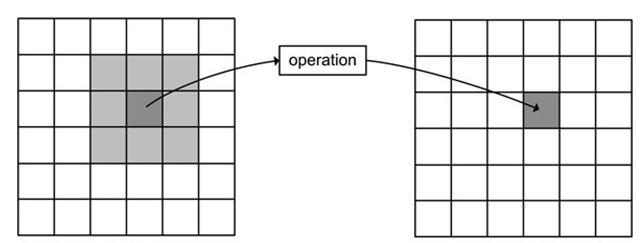
\includegraphics[scale = 0.5]{../../Images/Report_29_08_18/filter.png}
\end{figure}

Deve ser observado que, nessa implementação, o coeficiente de variação é calculado para amostras de uma dada banda de intensidade e, por isso, é dado por:
\begin{displaymath}
cv = \frac{ s }{ \overline{x} }
\end{displaymath}
em que $\overline{x}$ e $s$ são a média e o desvio padrão da amostra, respectivamente.

Uma característica relevante dos dados obtidos a partir da aplicação desse filtro a dados PolSAR é que esses obedecem a distribuição Gama, podendo variar apenas em relação ao valor dos parâmetros. Uma variável aletória obedece a essa distribuição quando sua função de densidade de probabilidade é:
\begin{displaymath}
f(x) =
\begin{cases}
\frac{ \beta^{\alpha} x^{\alpha - 1} }{ \Gamma(\alpha)} \exp(-\beta x), & \mbox{se x }>\mbox{ 0}\\
0, & \mbox{caso contrário.}
\end{cases}
\end{displaymath}
em que $\alpha$ e $\beta$ são parâmetros positivos e $\Gamma(\cdot)$ representa a função gama de Euler"
\begin{displaymath}
\Gamma(\alpha) = \int_{0}^{\infty} t^{\alpha - 1} \exp(-t) dt.
\end{displaymath}

\section{Visualização de imagens PolSAR}

A implementação desenvolvida fez uso dos recursos disponíveis na biblioteca \texttt{raster}, de modo que divergiu da implementação apresentada no relatório anterior somente no trecho de código que trata da equalização dos dados. Tal trecho foi substituído pelo seguinte:

\begin{verbatim}

parallel_cv <- function(x){ 
    localFun( x, x, ngb = dim, fun = function(a,b) ( sd(a)/mean(a) ))
}

beginCluster()

hhhh_cv <- clusterR(hhhh, fun = parallel_cv, filename="hhhh_cv.grd")
hvhv_cv <- clusterR(hvhv, fun = parallel_cv, filename="hvhv_cv.grd")
vvvv_cv <- clusterR(vvvv, fun = parallel_cv, filename="vvvv_cv.grd")

endCluster()

\end{verbatim}

A função \texttt{parallel}\textunderscore\texttt{cv} recebe um objeto RasterLayer e gera um outro com as mesmas dimensões e cujos valores em suas células são coeficientes de variação calculados para suas correspondentes no parâmetro. Esse coeficiente é calculado para uma dada célula a partir de uma matriz quadrada de ordem \texttt{dim} centralizada nessa. A implementação dessa funcionalidade foi feita utilizando \texttt{localFun}, a qual aplica funções a RasterLayers de forma localizada e sem manter o conjunto de dados que está processando integralmente na memória principal.

Contudo, afim de obter melhor desempenho, são utilizadas funcionalidades de \textit{multi-core computing} para dividir a execução de \texttt{parallel}\textunderscore\texttt{cv} entre os múltiplos núcleos de processamento disponíveis. Isso é feito pela função \texttt{clusterR}, a qual aplica ao objeto RasterLayer, de forma paralela, a função passada no parâmetro \texttt{fun}, armazena o resultado em arquivos no formato padrão Raster e retorna um objeto RasterLayer referenciando estes.

No entanto, para utilizar esse mecanismo é necessário criar previamente um objeto cluster por meio de \texttt{beginCluster}, e finalizá-lo quando não mais for necessário, o que é feito por \texttt{endCluster}.

Segue um resultado obtido a parir de dados \textit{multi-look}:

\begin{figure}[!h]
	\begin{center}    
		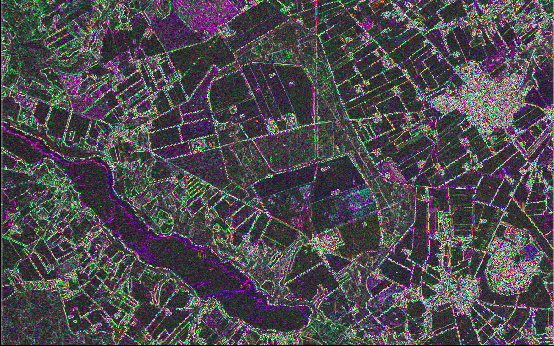
\includegraphics[width = 130mm, scale = 0.5]{../../Images/Report_29_08_18/foulum_cv_reduced.png} \\ 
 	\end{center}
\end{figure}

\newpage

\section{Análise de desempenho}

Para a analisar o desempenho da implementação desenvolvida utilizou-se um computador com 16GB de memória RAM, processador i7-7500U com 4 núcleos e frequência de 2.7GHz. Além disso, as matrizes extraídas para cálculo do coeficiente de variação foram de ordem 3 e durante a execução do filtro foram utilizados somente 3 núcleos de processamento.

Nessa análise, obteve-se o tempo decorrido durante a execução do filtro sobre objetos do tipo RasterLayer de diferentes dimensões e cujos os dados residiam em arquivos no formato padrão Raster. Além disso, os dados foram simulados, de modo que obedecem a distribuição contínua uniforme com parâmetros a = 0 e b = 1. Segue um gráfico com os resultados:

\begin{figure}[!h]
\centering 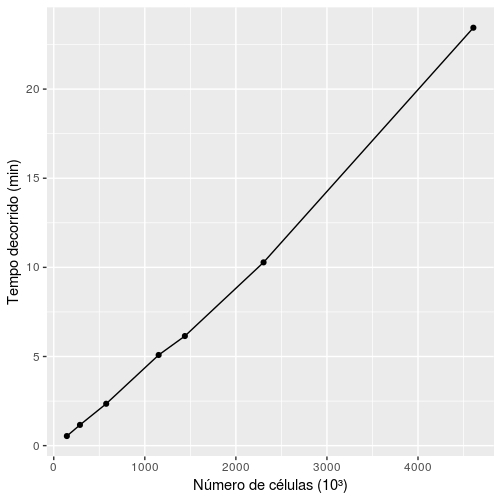
\includegraphics[scale = 0.7]{../../Images/Report_29_08_18/performance.jpeg}
\end{figure}

%Referências bibliograficas
%\bibliographystyle{unsrt}
%\bibliography{Bibliography/ref}

\end{document}
